\documentclass[10pt]{article}
\usepackage[T1]{fontenc}
\usepackage{lmodern}
\usepackage[margin=0.7in]{geometry}
\usepackage{amsmath}
\usepackage{microtype}
\usepackage{graphicx}
\usepackage{float}
\usepackage{booktabs}
\usepackage{enumitem}
\setlist[enumerate]{itemsep=2pt,topsep=3pt,leftmargin=1.5em}
\usepackage[font=small,labelfont=bf,skip=3pt]{caption}
\captionsetup[figure]{font=footnotesize}
\usepackage[dvipsnames]{xcolor}
\usepackage[colorlinks=true,linkcolor=MidnightBlue,citecolor=MidnightBlue,urlcolor=MidnightBlue]{hyperref}
\usepackage[capitalise]{cleveref}
\setlength{\parskip}{2pt}
\setlength{\parindent}{0pt}
\setlength{\intextsep}{6pt}
\makeatletter
\renewcommand\paragraph{\@startsection{paragraph}{4}{\z@}{1.0ex \@plus .3ex \@minus .2ex}{-1em}{\normalfont\normalsize\bfseries}}
\renewcommand\maketitle{\begin{center}{\large\bfseries\@title\par}\vspace{3pt}\@author\quad\textperiodcentered\quad\@date\end{center}}
\makeatother

\title{A negative singular-value power with matrix products only:\\[1pt]
\normalfont the two-track Newton--Schulz method, and why it is slow}
\author{Juntang Wang and V\'ictor Conchello}
\date{November 15, 2026}

% Coefficients (alpha, beta, gamma) of the Z step for p = -0.3, with Muon's (a, b, c) = (3.4445, -4.7750, 2.0315):
%   first iteration   ( 4.9125, -8.0324, 3.7790)
%   middle iterations ( 4.9915, -7.8279, 3.4157)
%   last iteration    ( 2.1740, -2.4723, 0.9797)   (here the X step is not needed)
% For p = -0.5: first (6.1049, -10.8787, 5.4076), middle (6.3927, -10.5965, 4.7000), last (2.1908, -2.9743, 1.2786).
% Start: X = Z = N / ||N||_F. The update is Z, rescaled as usual.
% LC: sv_power_lc and its coefficients in code/optsplit/optim/muon.py, branch two-track (all fitted sets: code/scripts/lc/final_coeffs.json).
% Fig. 1 (negative_p_method_lc.pdf): the LC5 set p-0.3_lc5_eps3.0e-03 applied to a single number sigma, step by step.

\begin{document}
\maketitle
\vspace{-0.8em}

\paragraph{The idea.} Muon replaces every singular value $\sigma$ of its momentum matrix $N$ by 1. Our exact runs replaced it by $\sigma^p$ and did best at $p=-0.3$, but they used a full decomposition (SVD), which made a training step 8 times slower. Muon's routine (Newton--Schulz) multiplies the matrix by a small polynomial of itself, several times. Each iteration pushes every $\sigma$ towards 1: a small one grows 3.44 times per iteration until it gets there. So by the end, $\sigma$ has been multiplied by about $1/\sigma$ in total. That total is what we need: $\sigma^p$ is $\sigma$ times $(1/\sigma)^{1-p}$.

\paragraph{The method.} Run Muon's routine on a matrix $X$ as usual and carry a second matrix $Z$ along. Both start as $N/\|N\|_F$ ($N$ divided by its norm, so that every $\sigma\le1$). In each iteration $X$ gets Muon's multiplier and $Z$ gets that multiplier raised to the power $1-p$. At the end the singular values of $Z$ are $\sigma^p$, and $Z$ is the update. With $M=XX^\top$:
\[ X\leftarrow(a\,I+b\,M+c\,M^2)\,X,\qquad Z\leftarrow(\alpha\,I+\beta\,M+\gamma\,M^2)\,Z. \]
$a,b,c$ are Muon's numbers. $\alpha,\beta,\gamma$ are chosen so that the second polynomial is close to the first one raised to $1-p$; their values for $p=-0.3$ are in this note's \texttt{.tex} source. $M$ and $M^2$ are shared, so $Z$ costs one extra matrix product per iteration.

\paragraph{Why it is slow.} ``Muon'' here always means \textbf{5 iterations of 3 matrix products: 15 products}. The two-track method takes 4 products per iteration (3 in the last one, which skips $X$). With the same 5 iterations that is 19 products and 1.4 times Muon's time, so the second matrix is not the main problem. The problem is the number of iterations. Each one lowers the smallest $\sigma$ that gets up to 1 by only a factor 3.44. Muon stops after 5, so singular values below about $10^{-3}\,\|N\|_F$ never get up to 1. Our exact runs applied $\sigma^p$ down to a millionth of the largest $\sigma$, and that takes 12 iterations (\cref{tab:cost}).

\paragraph{LC (sum of iterates).} LC$K$ (linear combination, $K$ steps) runs $K$ Newton--Schulz steps like Muon's from $X_0=N/\|N\|_{S_8}$ and returns a fixed weighted sum of the iterates:
\[ X_{k+1}=(a_kI+b_kM_k+c_kM_k^2)\,X_k,\quad M_k=X_kX_k^\top,\qquad \text{update}=\textstyle\sum_{k=0}^{K} w_kX_k. \]
\begin{itemize}[itemsep=2pt,topsep=3pt,leftmargin=1.5em]
\item \textbf{Why it works.} Write $X_0=USV^\top$. A step keeps $U$ and $V$ and maps each singular value $\sigma$ to the odd polynomial $a_k\sigma+b_k\sigma^3+c_k\sigma^5$, so $X_k=U\varphi_k(S)V^\top$, where $\varphi_k$ applies the first $k$ of these polynomials in turn. The sum has singular values $g(\sigma)=\sum_k w_k\varphi_k(\sigma)$, again an odd polynomial, fitted so that $g(\sigma)\approx\sigma^p$ (a constant factor does not matter: the update is rescaled). \Cref{fig:lc} shows the $\varphi_k$ and $g$ for LC5.
\item \textbf{Fit.} Unlike Muon, each step has its own $a_k,b_k,c_k$. These and the $w_k$ are fitted once, offline, to minimize the worst relative error to $\sigma^p$ on a grid of $\sigma\in[\varepsilon,1]$ (\texttt{code/scripts/lc/}).
\item \textbf{Norm.} The Schatten 8-norm $\|N\|_{S_8}=\|(NN^\top)^2\|_F^{1/4}$ costs nothing (step 0 forms $NN^\top$ and its square anyway). Like $\|N\|_F$, it is at least the largest singular value, but it is closer to it, so fewer singular values fall below $\varepsilon$.
\item \textbf{Limit.} Near 0 an odd polynomial is a line through 0, so below $\varepsilon$, $g$ falls to 0 instead of growing like $\sigma^p$. Each extra step (3 products) moves $\varepsilon$ about 3 times lower: LC5 is within $\pm13\%$ of $\sigma^p$ above $3\cdot10^{-3}$, LC12 within $\pm16\%$ above $2\cdot10^{-6}$. \Cref{tab:cost} and \cref{fig:map} instead give $\sigma$ as a fraction of $\|N\|_F$, which puts the largest singular value at about 0.4.
\item \textbf{Cost and origin.} 3 products per step, so $3K$ in all (LC5: Muon's 15); the sum adds none. We designed LC; the same family appeared earlier in \href{https://varunneal.github.io/essays/spectral-powers}{Srivastava's blog post}, but the coefficient sets are ours.
\end{itemize}

\begin{figure}[H]
\centering
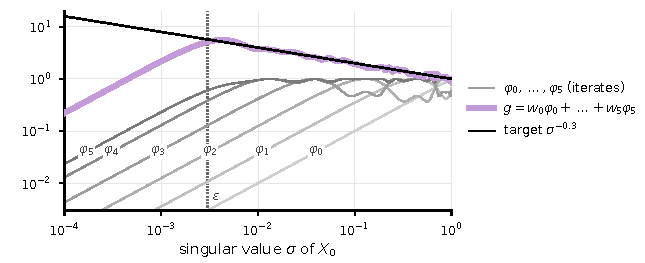
\includegraphics{negative_p_method_lc.pdf}
\caption{LC5 for $p=-0.3$, computed by applying its five steps to a single number $\sigma$. Thin: $\varphi_0,\dots,\varphi_5$, the singular values of $X_0,\dots,X_5$. Thick: their weighted sum $g$, with $w=(-0.89,-1.29,-1.63,-0.91,-11.76,\,16.28)$. It stays within $\pm13\%$ of $\sigma^{-0.3}$ (black) above $\varepsilon=3\cdot10^{-3}$; below, it falls in proportion to $\sigma$.}
\label{fig:lc}
\end{figure}

\begin{table}[H]
\centering
\footnotesize
\caption{Cost for $p=-0.3$. Reach: the singular value, as a fraction of $\|N\|_F$, where the update falls to half its target ($\sigma^p$; 1 for Muon). Time: on a laptop, relative to Muon. GPU: ms per training step (exact SVD: 1072; AdamW takes as long as Muon). Error: relative distance to the exact update on synthetic matrices (0 is identical, above 1 unrelated); most of the exact update sits in the very small singular values. The last two-track iteration grows small $\sigma$ less (it only corrects), hence a shorter reach than Muon's at 5.}
\label{tab:cost}
\begin{tabular}{l cccccc}
\toprule
 & iterations & reach & products & time & GPU & error \\
\midrule
Muon ($p=0$) & 5 & $1\cdot10^{-3}$ & 15 & 1 & 129 & 1.2 \\
two-track & 5  & $2\cdot10^{-3}$ & 19 & 1.4 & 146 & 1.2 \\
two-track & 8  & $5\cdot10^{-5}$ & 31 & 2.3 & 164 & 1.0 \\
two-track & 12 & $4\cdot10^{-7}$ & 47 & 3.5 & 186 & 0.1 \\
LC5  & 5  & $6\cdot10^{-4}$ & 15 & 1.0 & 135 & 1.2 \\
LC8  & 8  & $4\cdot10^{-5}$ & 24 & 1.5 & 154 & 1.0 \\
LC12 & 12 & $4\cdot10^{-7}$ & 36 & 2.2 & 170 & 0.2 \\
\bottomrule
\end{tabular}
\end{table}

In training (MSE loss; final validation loss, mean of 3 runs), the exact $p=-0.3$ beats Muon: 0.5626 against 0.5663. LC5 and two-track with 5 iterations end worse than Muon (0.576 and 0.579), so the gain needs the very small singular values. LC12 matches the exact run (0.5624) at 1.3 times Muon's GPU step time.

\paragraph{Is $X$ needed?} With these formulas, yes: $Z$'s multiplier is computed from $X$. An iteration on $Z$ alone (each $\sigma$ approaches 1 slowly, at a distance proportional to $\sigma^p$) needs 60 products to come close to two-track with 12 iterations (47): no gain.

\begin{figure}[H]
\centering
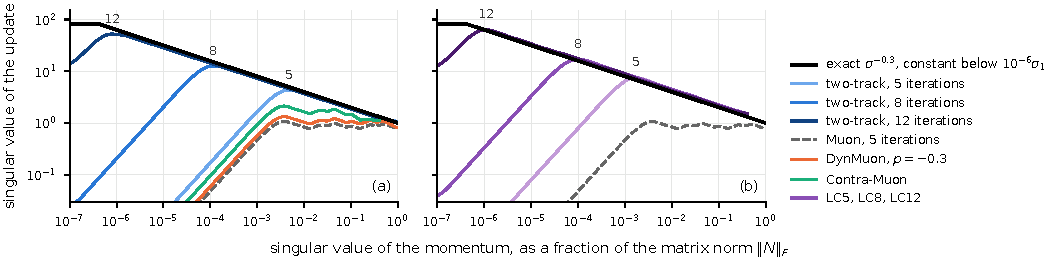
\includegraphics[width=\linewidth]{negative_p_method_map.pdf}
\caption{The update's singular value against the momentum's ($\sigma_1$, the largest, is drawn at $0.4\,\|N\|_F$; oscillations smoothed). (a): published variants at Muon's cost, \href{https://arxiv.org/abs/2605.17109}{DynMuon} and \href{https://nilin.github.io/contra-muon-and-soft-muon}{Contra-Muon}, stay close to Muon's flat shape. (b): LC5, LC8 and LC12, with the coefficients used in training.}
\label{fig:map}
\end{figure}

\end{document}
